\documentclass[11pt]{amsart}
\usepackage{geometry}                % See geometry.pdf to learn the layout options. There are lots.
\geometry{letterpaper}                   % ... or a4paper or a5paper or ... 
%\geometry{landscape}                % Activate for for rotated page geometry
%\usepackage[parfill]{parskip}    % Activate to begin paragraphs with an empty line rather than an indent
\usepackage{graphicx}
\usepackage{amssymb}
\usepackage{epstopdf}
\usepackage{enumerate}
\DeclareGraphicsRule{.tif}{png}{.png}{`convert #1 `dirname #1`/`basename #1 .tif`.png}
\setlength{\parindent}{0in} % no paragraph indent

\usepackage{fancyhdr}
\pagestyle{fancy}
\lhead{\footnotesize \parbox{11cm}{STAT 434 Data Analysis} }
\rhead{\footnotesize \parbox{11cm}{Max Scheiber and Ruslan Zagatskiy} }

\title{STAT 434 Data Analysis - Max Scheiber and Ruslan Zagatskiy}
\date{11.25.2013}

\begin{document}
\maketitle
\section{Overview}
Our goal was to explore the relationship between the NSA scandals of 2013 and securities of related tech sector stocks. \\

\section{Raw data to polished data}
We obtained consolidated trade data from Wharton Research Data Services (WRDS) for Google (GOOG), Apple (AAPL), Microsoft (MSFT), and Facebook (FB) for the January 1st, 2013 through July 31st, 2013 timespan. These consolidated datasets contain average execution prices and total shares volume a few times each second. We chose these stocks because they were the ones identified in the NSA's leaked slide deck. \\

To make data analysis more manageable, we converted this data into hourly buckets from 9am to 3pm, inclusive. We did this by taking the average execution price over each bucket, equally weighted within the bucket. (For the final presentation, it may be better to volume-weight this mean). We also took volume sums for each bucket. \\

We then created a basket of tech stocks by taking the equal-weighted average of each bucket of all stocks considered. The reason for doing this was to enhance our signal-to-noise ratio; this basket would minimize the effects in securities pricing and volatility of, say, one company's earnings report, while confirming sector-wide trends. \\

Within this basket, we computed percent returns, which allowed us to compute a scale-independent moving volatility. We currently measure volatility from a given time bucket over the previous 30 time buckets. Given that there are seven buckets per day, we see our volatility measure cover a duration of just over four days. (For the future, we may wish to model volatility with an exponential smooth.) \\

\newpage
\section{Google analysis}
Before performing analysis on the basket of stocks, we performed some basic analysis of Google's returns. \\

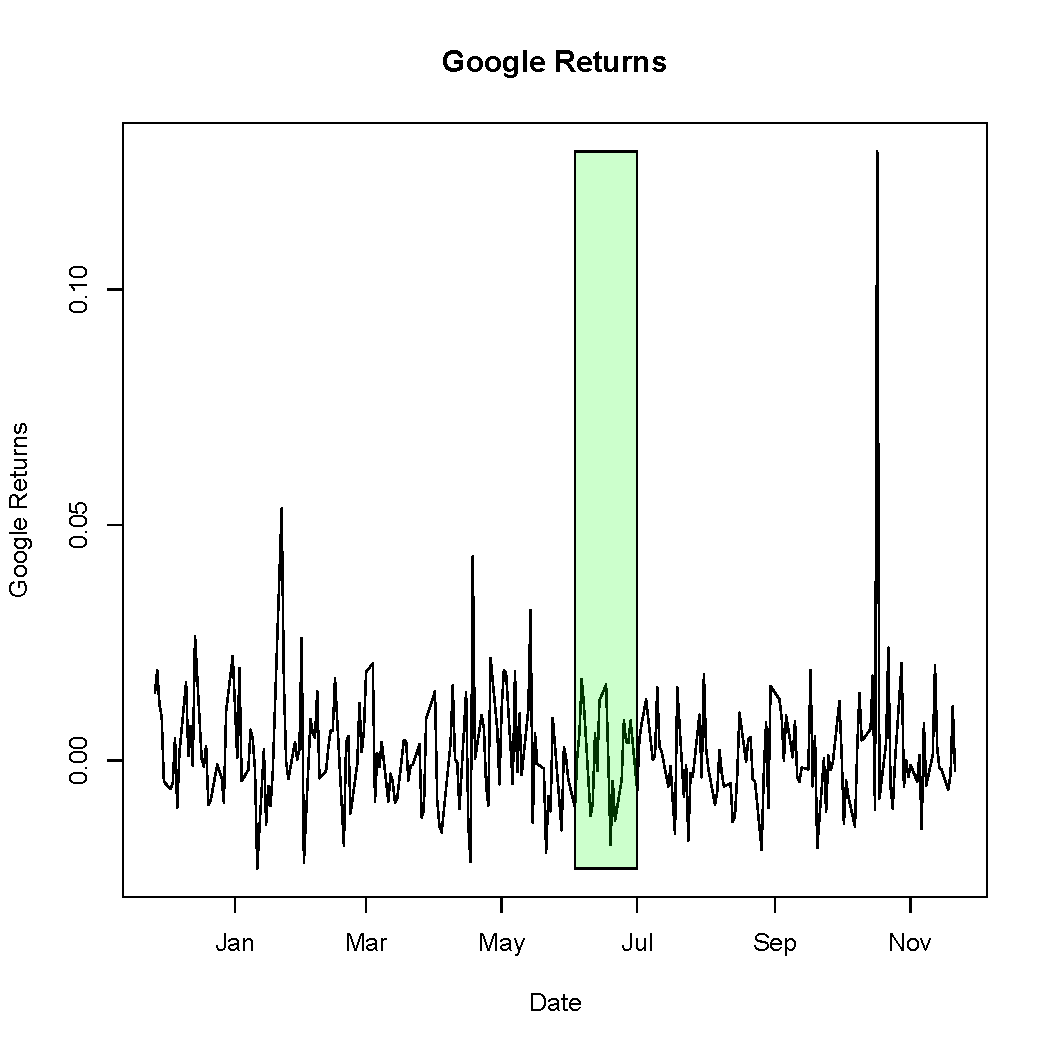
\includegraphics[scale=0.4]{goog_returns_11_25.pdf} \\

Immediately, we can see that Google did not really have any outliers in its return over the summer. Its main spikes seem to come from its earning reports, implying that the market did not judge the NSA scandals to really affect Google. \\

We next look at Google's hourly volatility throughout June, which is when the majority of the NSA leaks happened. It initially seems obvious via eyeballing that Google's volatility spiked on June 6th (the date of \textit{The Guardian}'s first leak) and June 20th (the date of \textit{The Guardian}'s second leak). \\

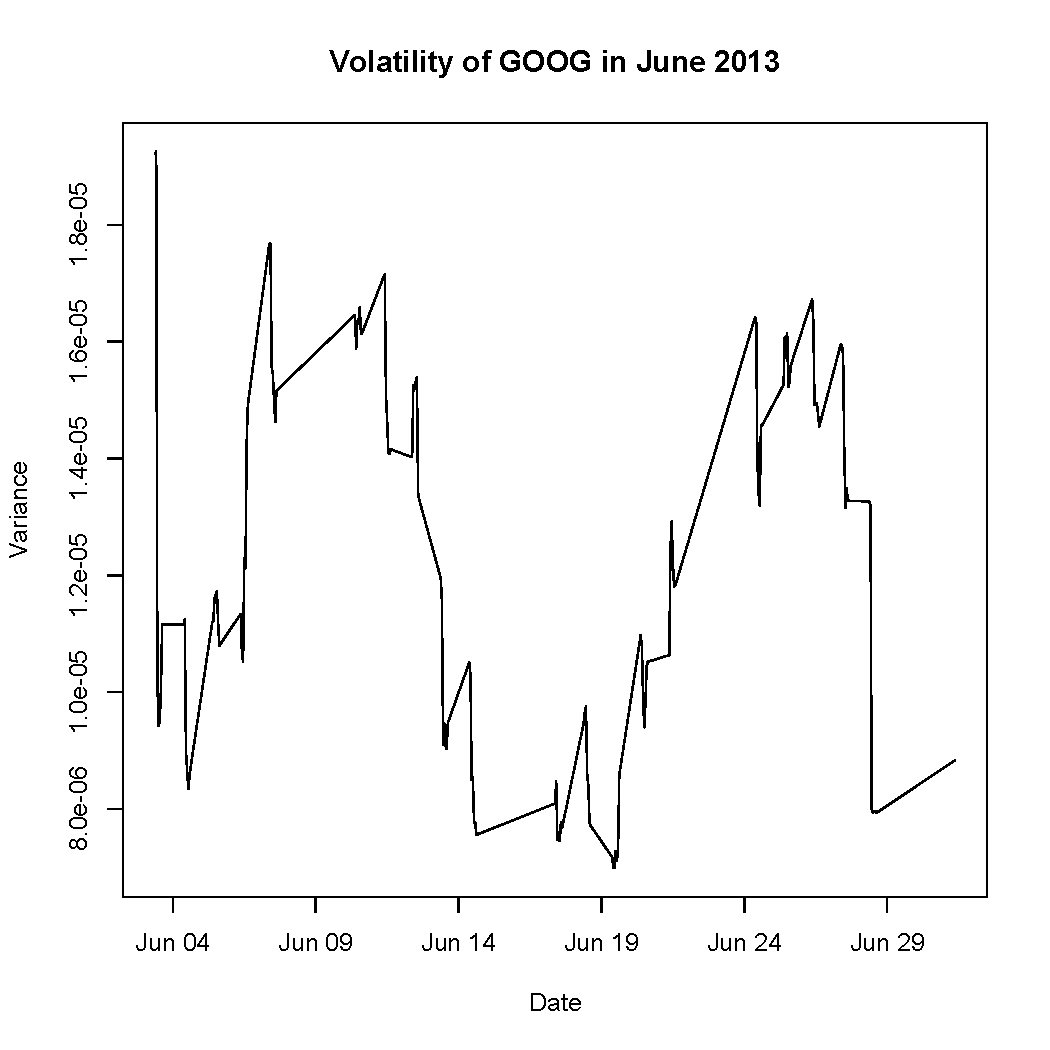
\includegraphics[scale=0.4]{goog_vol_zoom_11_25.pdf} \\

However, in context, these spikes are extremely minimal. Let us, for example, plot volatility throughout 2013. \\

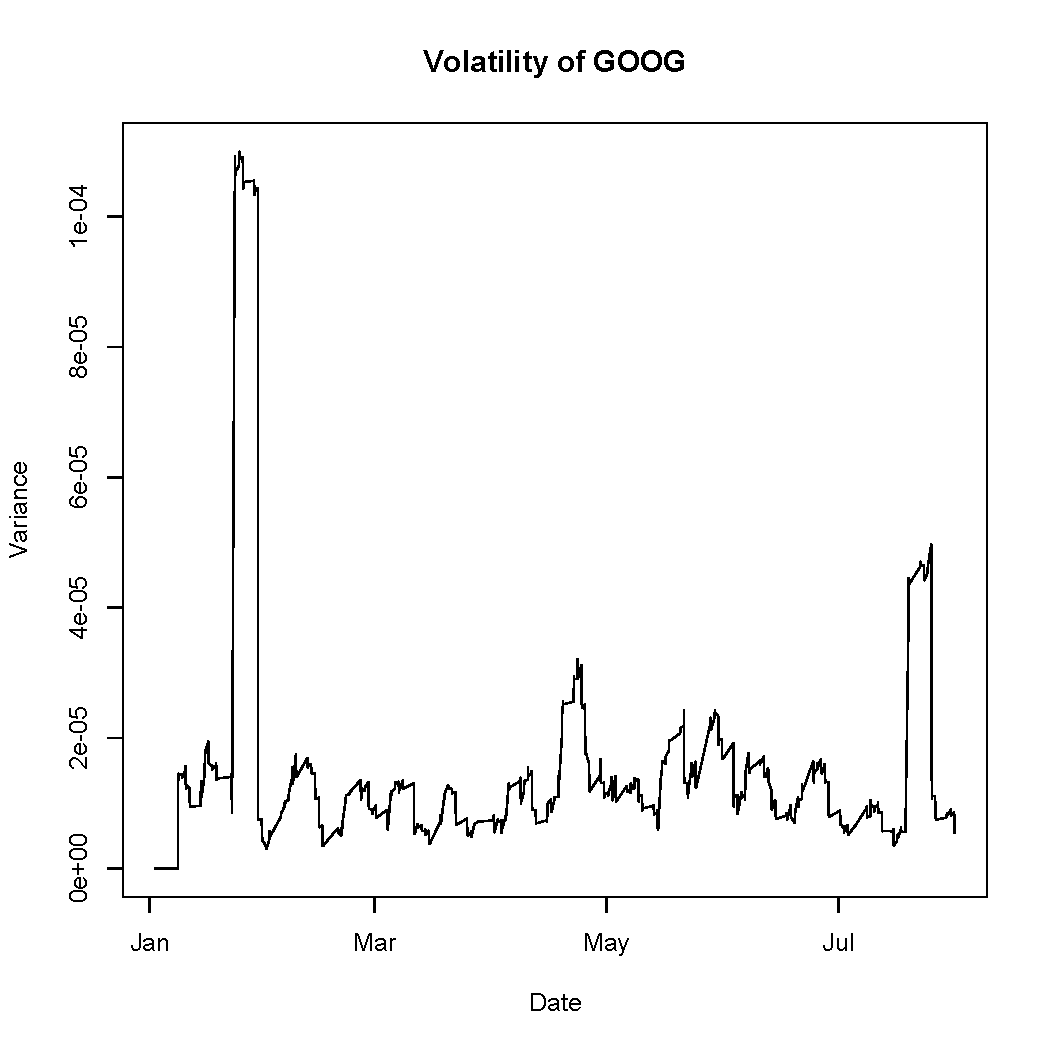
\includegraphics[scale=0.4]{goog_vol_11_25.pdf} \\

Any June spikes that could be related to the NSA do not look very significant in the context of Google's volatility throughout the year. While it is ostensible that these small June spikes may indeed have occurred as a result of the NSA scandal, this seems to be an early indicator that our hypothesis may not hold.

\newpage
\section{Tech sector basket analysis - full data set}
For further confirmation, we now look at the full tech sector basket as discussed in section 2. \\

To check for any sort of heteroskedasticity, we plot squared returns of the basket. Note that while we also
applied our moving volatility model to basket data, the plot of squared returns provides a simpler visual 
analysis that leads to the same conclusions.\\

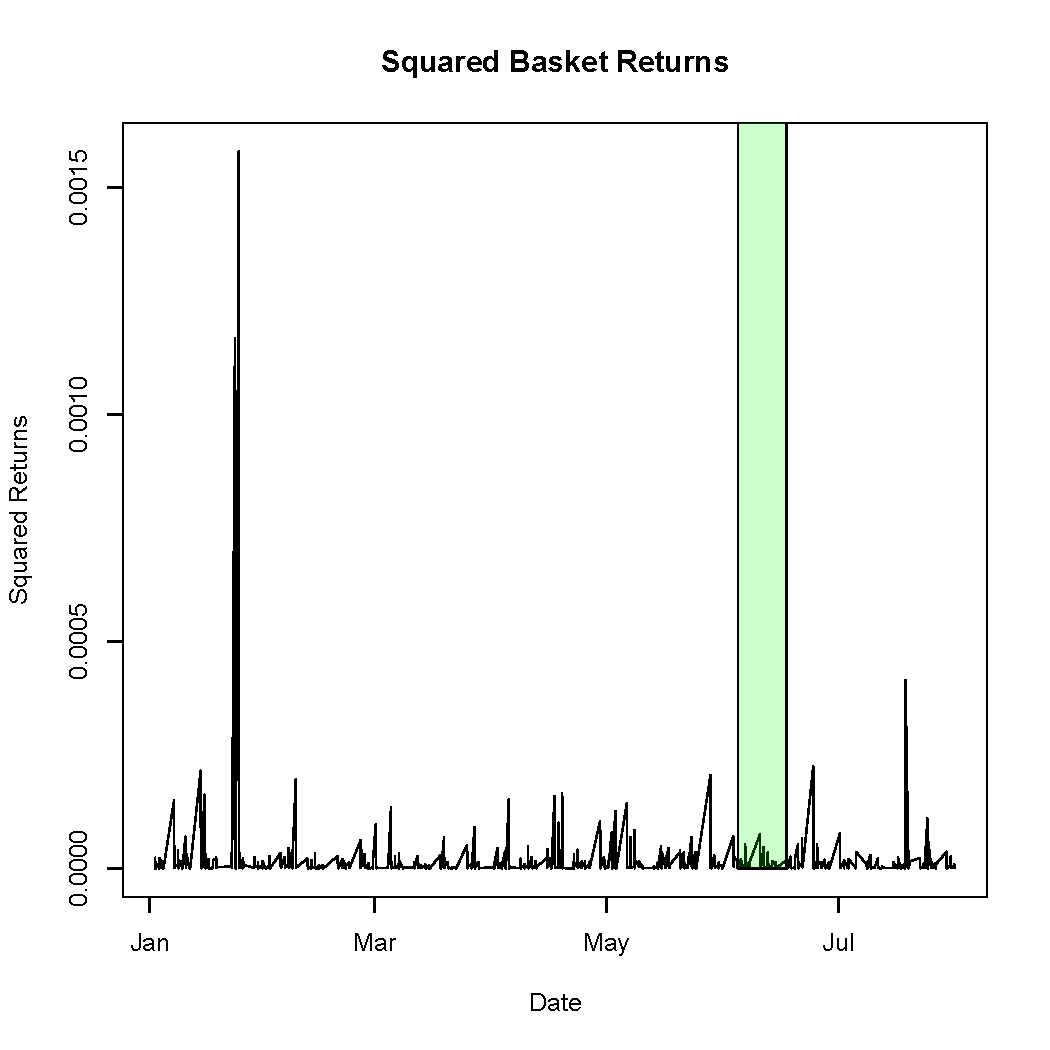
\includegraphics[scale=0.4]{basket_sq_returns_11_25.pdf} \\

\newpage
While the basket's 2013 squared returns have some unusual spikes,  it looks generally stable. More rigorously, we considered an ARCH(1) model for the basket's returns. The model's first coefficient is statistically insignificant, implying homoskedasticity. Of course, testing just an ARCH(1) is not sufficient. Next we look at an ARCH(8), where we find that the 6th and 7th lags are significant. Finally, we consider a GARCH(1,1), which is essentially equivalent to an 
infinte order ARCH. The significance of both the ARCH(alpha1) and GARCH(beta1) terms confirms heteroskedasticty
in the basket return variance.  \\



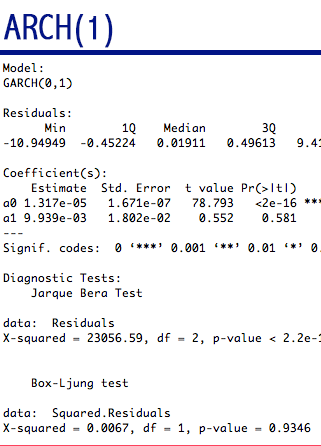
\includegraphics[scale=0.5]{arch1_basket_11_25.png} \\
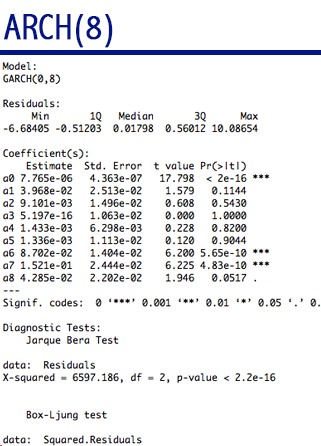
\includegraphics[scale=0.5]{arch8_basket_12_2.png} \\
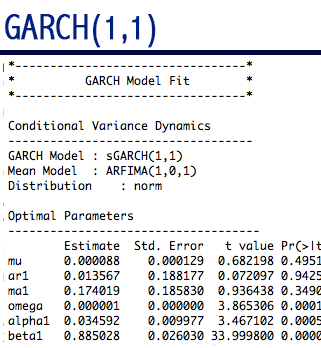
\includegraphics[scale=0.5]{garch11_basket_12_2.png} \\

\newpage
\section{June indicator variables}

The discovery above is unsurprsing - heteroskedastic variance is a common feature of financial returns. A more interesting question is whether the NSA leaks, independent of other events, impacted volatility. \\

One approach is to regress using an indicator variable. We set an indicator variable to be true for all buckets on June 6th, the day of the first NSA leak, and we set another indicator variable to be true for all buckets on June 20th, the day of a large second NSA leak. We test the significance of these indicators first for our full data set and find that neither have t-Statistics large enough to reject the null that they have no impact. \\

The section above considers long-run impact of the NSA leaks on the volatiltiy of our tech basket. However, it is
also worth considering short-run volatility changes centered around the time of the leaks. We first consider the month of June since that is when the leaks began. A plot of squared returns suggests that there is some increased volatiltiy towards the end of June, particularly around June 21st (our model's volatility is lagged by about 3 days). This is confirmed by a GARCH(1,1), which has significant coefficients for lagged variance and lagged squared error terms. \\

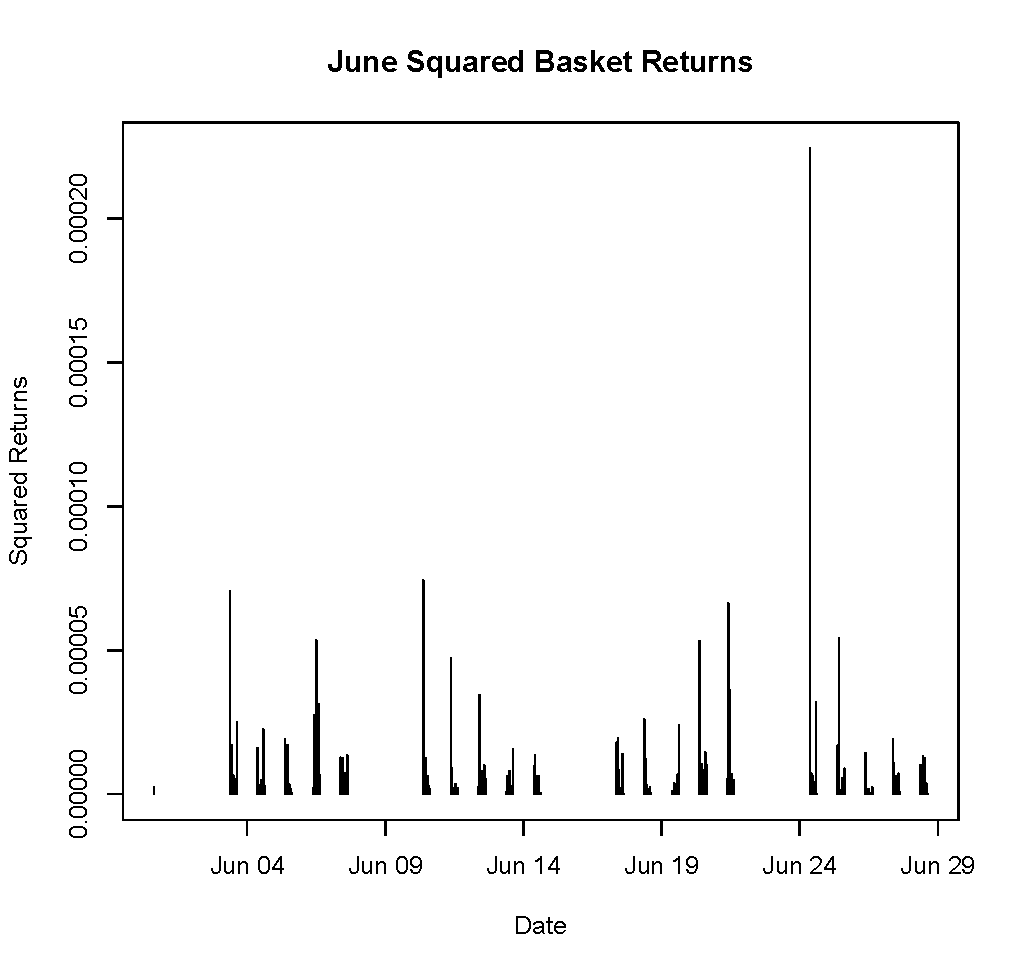
\includegraphics[scale=0.6]{june_squared_basket_ret.pdf} \\

\newpage
The result of these regressions is that only the June 20th leak is statistically significant for June volatility. The June 6th indicator does not have significant explanatory power for volatility in June or in all of 2013. It is arguable that \textit{The Guardian}'s second leak did spur more volatility in the market, but this washes out in the long run due to other similar events that affect the tech sector. There are a variety of possible explanations for the significance of June 20th versus the  null effect of June 6th, but these are purely speculative. \\

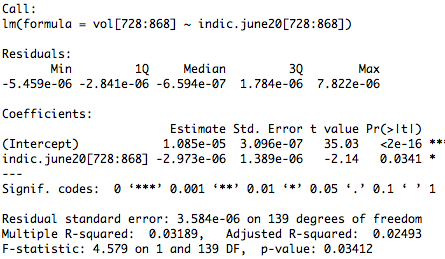
\includegraphics[scale=0.6]{june_20_june_11_25.png} \\

\newpage
It is worth highlighting that June is not a particularly volatile month. This raises the question of whether these spikes were truly caused by the NSA leak or are just a product of the basket's natural long-run volatility; June's volatiltiy looks fairly tame in the grand scheme of things. This is illustrated in the plot below, which compares June (black) with three random months. If anything, June's volatility is lower than the random months. What this is suggests is that \textit(even if) the NSA leak caused a surge in volatility, the change was so small that it is hardly worth mentioning. \\

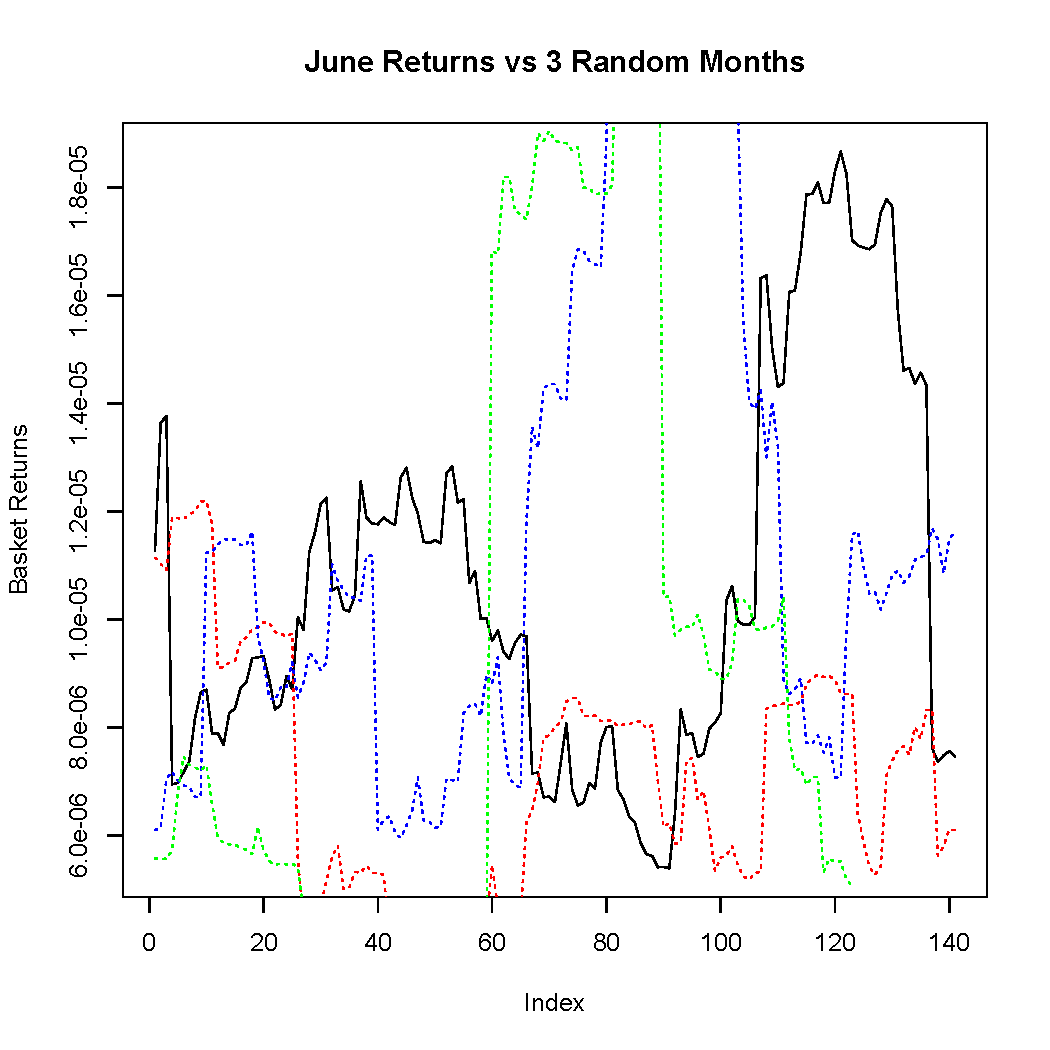
\includegraphics[scale=0.7]{june_3_months.pdf} \\

\newpage
\section{July indicator variables}
Next, we will consider July. A plot of squared July returns suggests a volatility spike sometime around July 18th. This is confirmed by a basic ARCH(1) model. \\

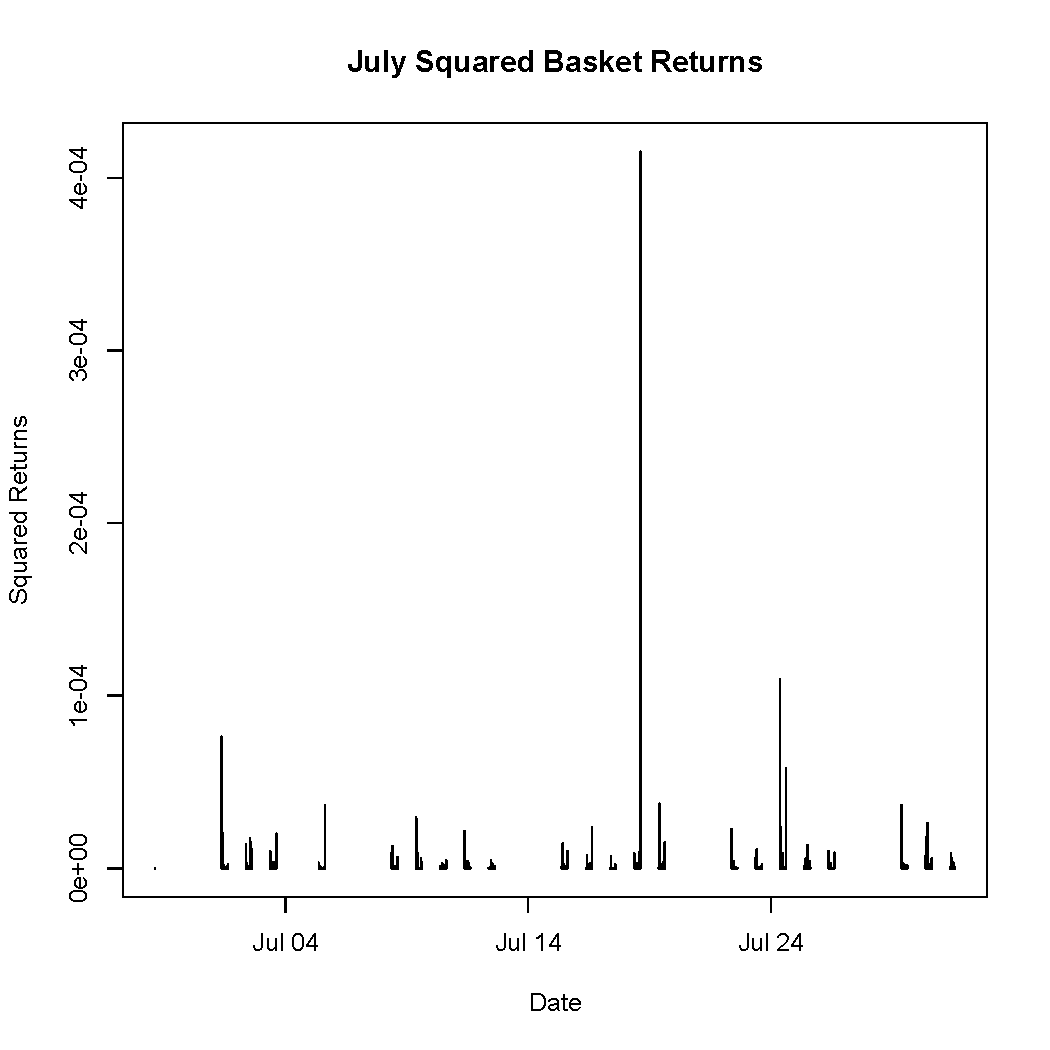
\includegraphics[scale=0.6]{july_squared_basket_ret.pdf} \\

While this initially seeming promising, it is worth noting that all of our companies had earnings reports at approximately those dates. Historically, company earnings reports have a large impact on volatility; investors are eager to adjust their portfolios based on the release of new public information. The plot below shows the squared returns of our four companies (colored) and the basket squared returns. The spikes in the company volatities are likely casued by their respective earnings releases; these combine to see the volatility spike in the basket. \\

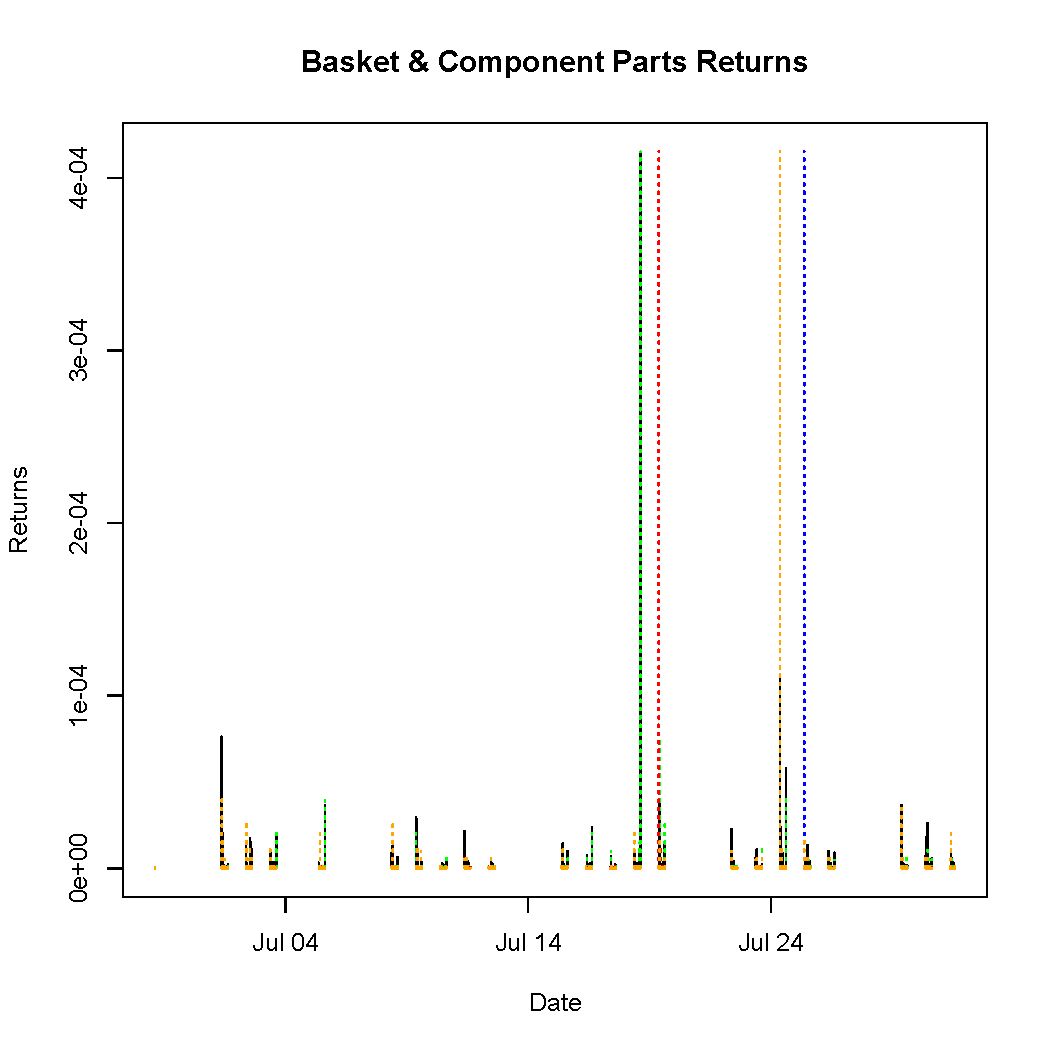
\includegraphics[scale=0.5]{july_earnings.pdf} \\

Finally, we can note that July volatility was not particularly large relative to other months in 2013. A plot comparing July volatility to the volatility in 3 random months is shown below. The results here are similar to those of June: even if the NSA leaks did have an effect, it was so small that it was hardly worth noticing. \\

 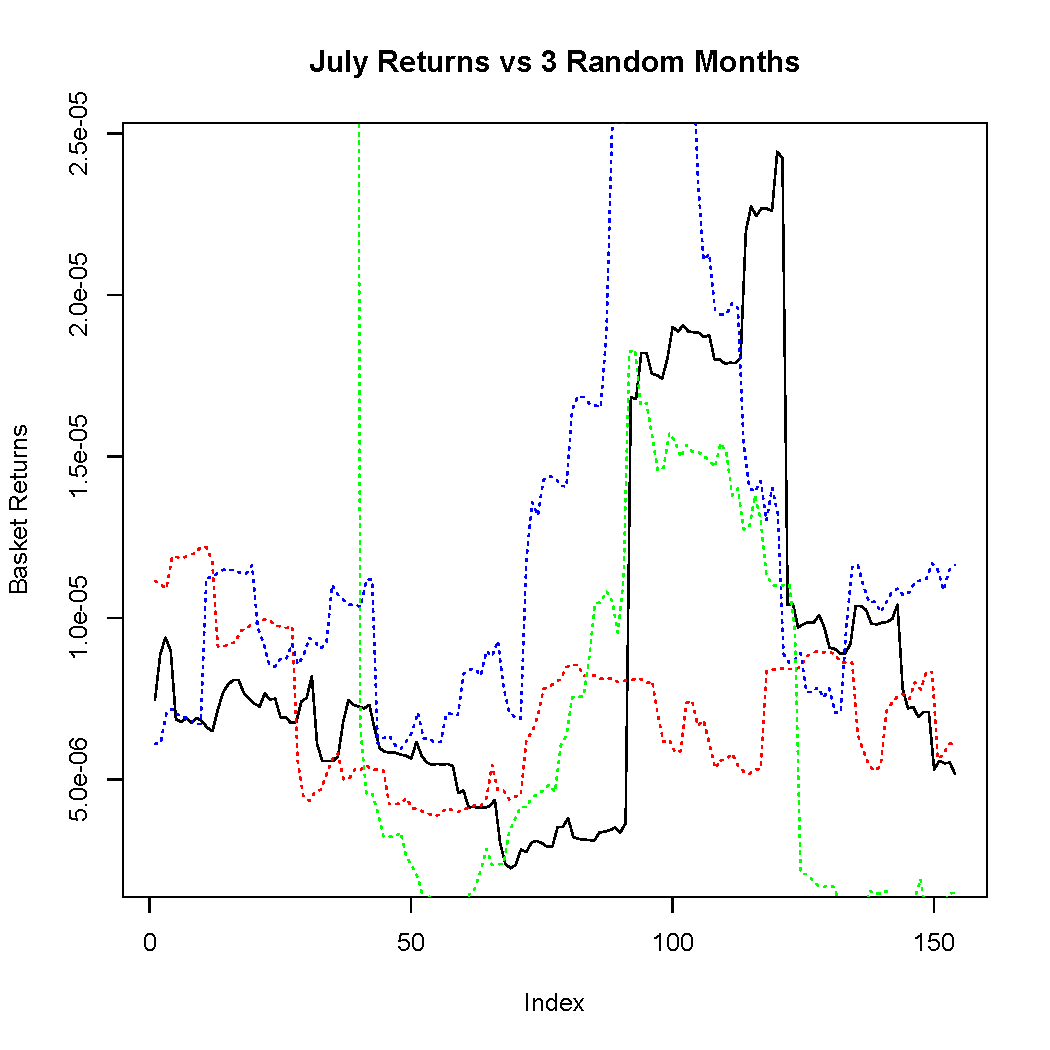
\includegraphics[scale=0.5]{july_3_months.pdf} \\

\newpage
\section{Volume}

So far, our volatility analysis hasn't worked out very well - we have just one probable date: June 20th. Now, let's look at another measure of market interest - volume.  \\

Let's take a look at volume for our entire data set, with June - end of July highlighted. Overall, we're seeing a lot of fluctuations in volume across the board, but our window from June - end of July looks particularly volatile. 

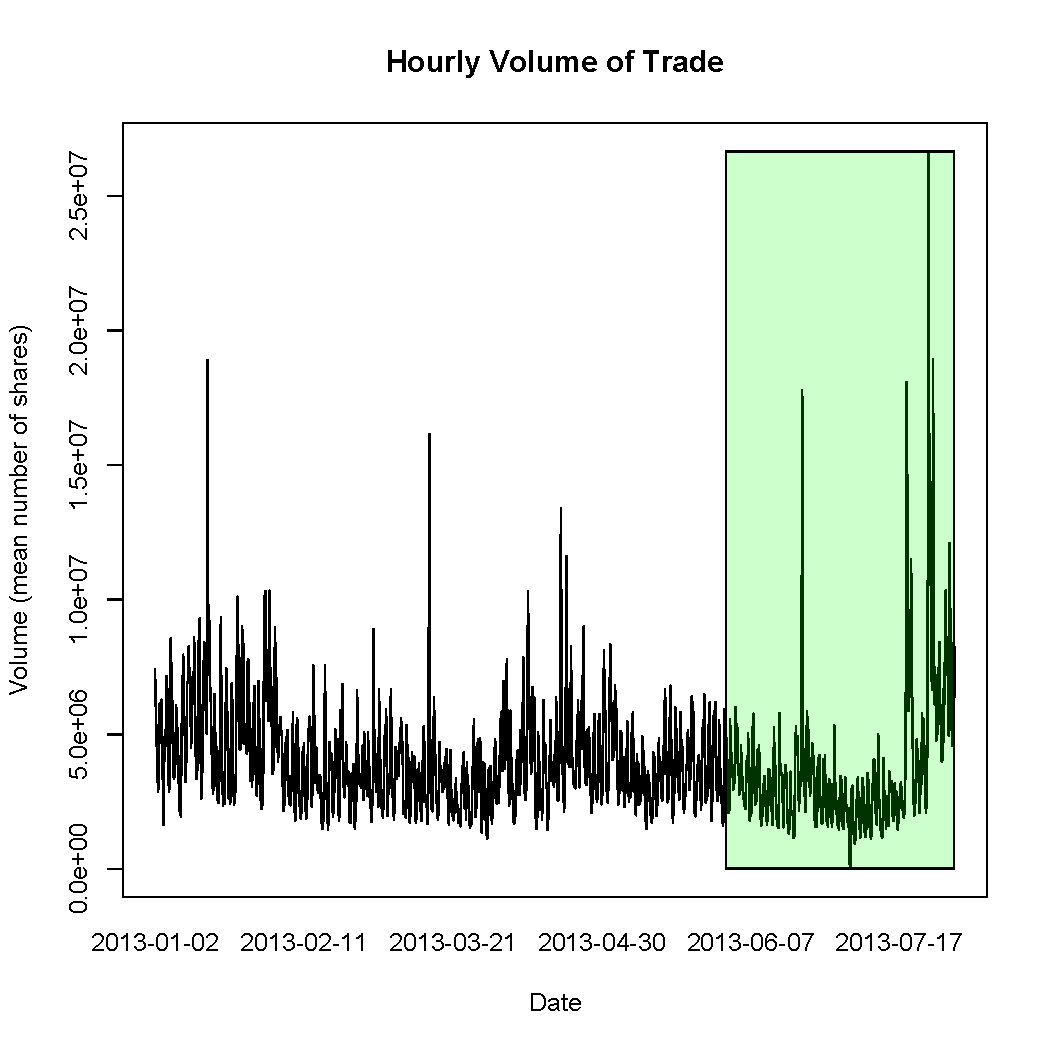
\includegraphics[scale=0.7]{june_july_volume.pdf} \\

\newpage

Let's start by taking a look at June in particular, we notice that somewhere around June 20th has large spike in volume. Below is a plot of June voume (black) and volatility (red) - clearly there's a large correlation between the two. This confirms our hypothesis that June 20th may have been very important for the market - at least in the ultra short horizon of a day or two in June. \\

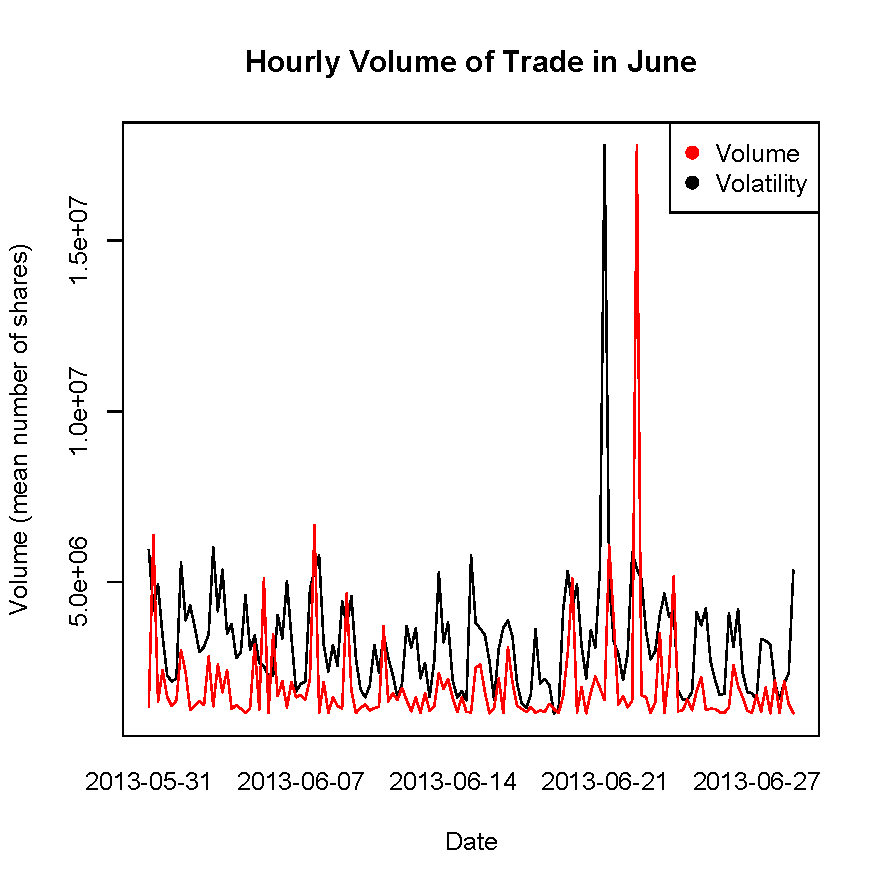
\includegraphics[scale=0.5]{june_volume_volatility.pdf} \\

\newpage

Now let's take a look at July. Overall, it looks like June 15th - 30th has a lot of volatiltiy in the volume. These results are similar to those we found for the volatility in the returns and are likely linked to the earnings reports for the respective companies, not an NSA leak. \\

In particular, Google and Microsft had their reports on the 18th, while Facebook and Apple had theirs on the 24th. \\

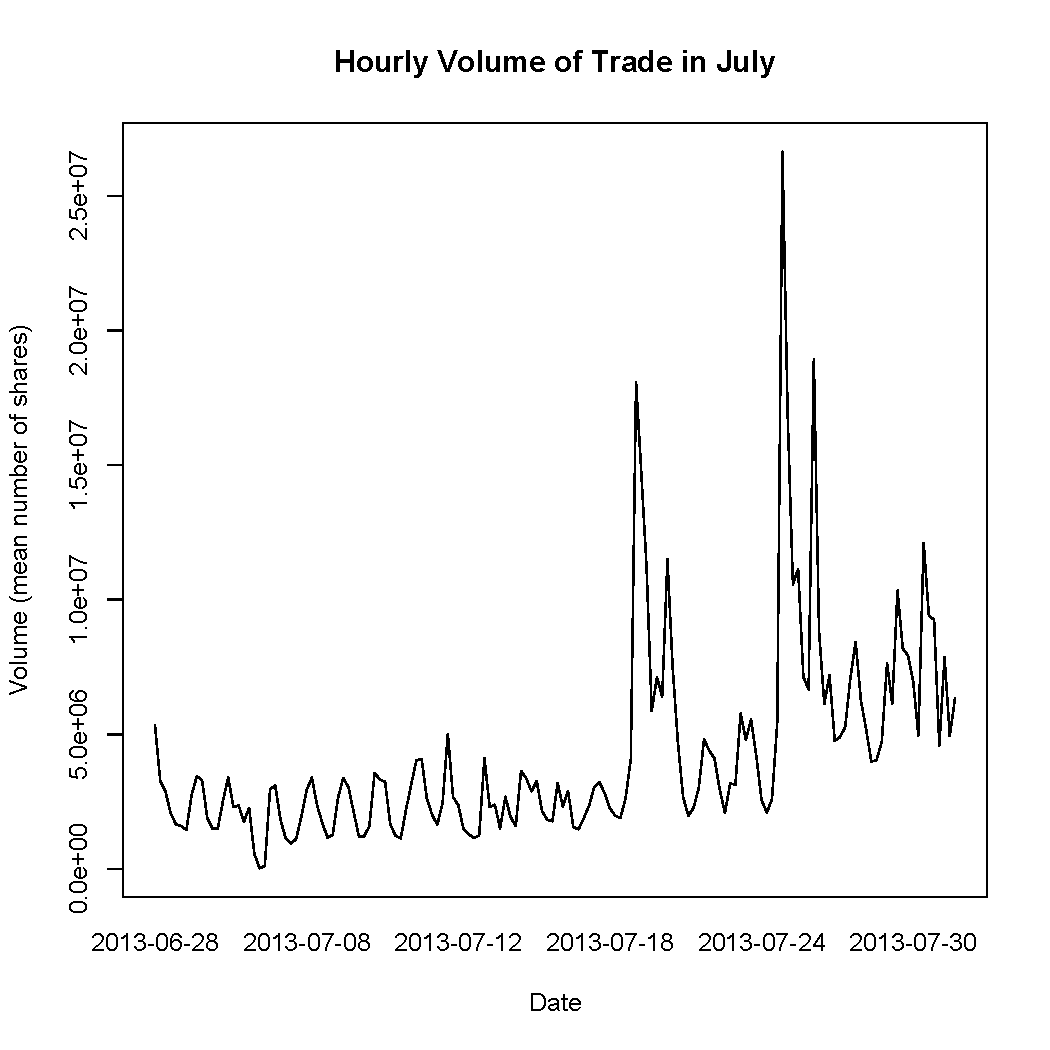
\includegraphics[scale = 0.5]{july_volume.pdf} \\


\newpage
\section{To come}

At this point we've rejected all dates except June 20th. We'll need to determine whether the spike in volatility/volume on the 20th was due to an NSA leak or some other event.  \\


\end{document}  